\begin{itemize}
    \item Beschreibt die Grundüberlegungen der realisierten Lösung (Konstruktion/Entwurf) und die Realisierung als Simulation, als Prototyp oder als Software-Komponente etc.
    \item Hier beschreiben Sie Ihre gemachte Arbeit. Dazu braucht es eine Beschreibung des Vorgehens, aller Arbeitsschritte usw.
    \item (Definiert Messgrössen, beschreibt Mess- oder Versuchsaufbau, beschreibt und dokumentiert Durchführung der Messungen/Versuche)
    \item Bildmaterial erleichtert das Verständnis.
    \item (Experimente)
    \item Immer mit Aufbau und Vorgehen; Bildmaterial erleichtert das Verständnis.
    \item (Lösungsweg)
    \item Inkl. theoretische Herleitung der Lösung
    \item (Modell)
    \item (Eingesetzte Software)
    \item Die Funktionen von verwendeten Computerprogrammen zu Simulationszwecken, Berechnungen etc. sollen beschrieben werden. Dies soll aber in Worten, Formeln und geeigneten Darstellungen (z.B. Fluss- diagrammen) geschehen. Allfälliger Programmcode ist in einem Anhang zu dokumentieren.
    \item (Tests und Validierung)
\end{itemize}

This chapter describes which approaches and methods have been used to solve the problem to find algorithms which calculate the optimum path on a racetrack.

\begin{figure}[H]
    \centering
    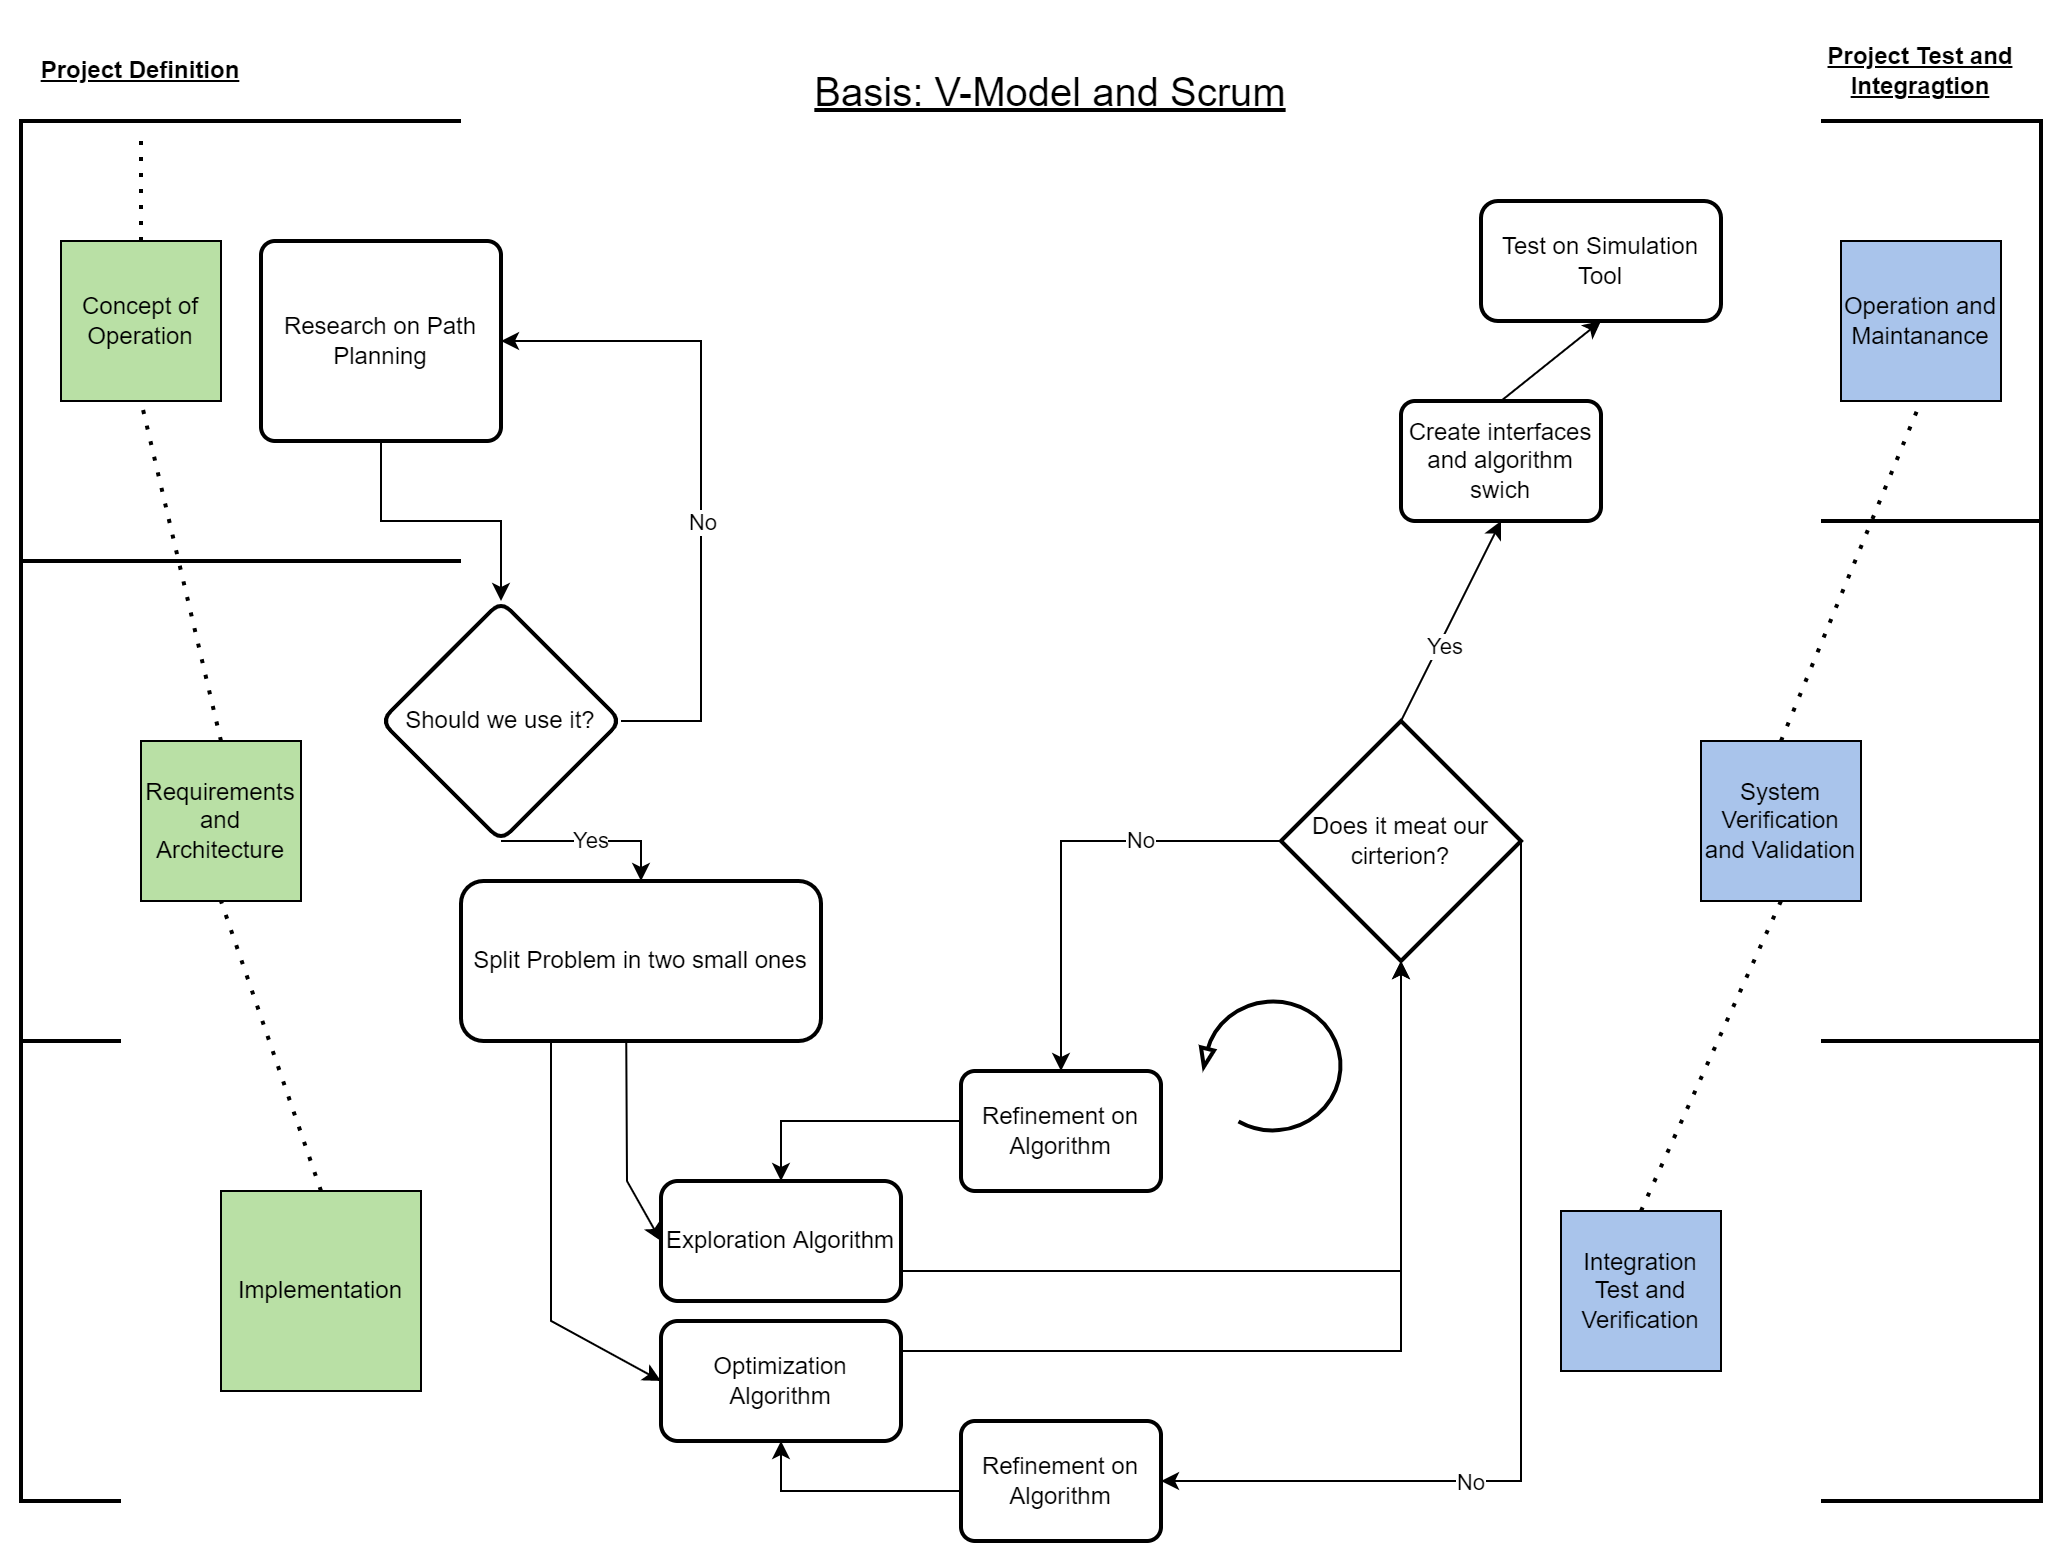
\includegraphics[width=\columnwidth]{High_Level_Project_Overview.png}
    \caption{The high level project overview gives an illustration which approaches and methods have been used to realize the project.}
    \label{fig:High Level Project Overview}
\end{figure}

\section{Marco's Proposal}
\begin{itemize}
    \item Anfangs High Level Overview Mischung, Kapitel ersichtlich was kommt Flussdiagram (um dieses haben wir dann die Prozessmethoden)
    \item Vorgehensmethode => Kanban und Scrum, maybe V-Model?
    \item Setup technisch, lokale Linux VM, ROS Installation, VS Code als IDE, GitHub Repos, GitHub Actions CI/CD (maybe?), Deployment Architektur
    \item Overview Architektur ROS und Code, Grundüberlegung => Path Planning Package in ROS, Prototyp Architektur zeigen, Explo und Opt Algos, erhaltet Input und sendet Input
    \item Messages (interfaces und fszhaw msgs) (System aussen)
    \item Path Planner Node
    \item Exploration Algorithm
    \item Optimization Service Node
    \item Optimization Algorithm
    \item Verifikation und Validierungen (Code Reviews, Fehlerfälle: Cones gehen verloren, Cones andere Seite entdeckt, allg Fehlerannahmen)
    \item Testing mit Maps, Cone Publisher und Planned Trajectory Subscriber (mocks), utils wie track plotter, trackconfig
    \item Setup eher im Projektanhang: Weekly meetings, Review every other week, Mitarbeit mit anderen BA Teams in Driverless und gesamt Verein (Working Saturday, Hilfe im Workshop, Ausstellung Conecto ZHAW)
    \item In Resultate Kapitel, Vergleich erste Algorithmen und Versuche: erste Überlegungen und Tests, alter path planner zhaw, dann densify und interpolate, rrt max hamburg, komplexer algo à la ultimate und dann jetzige implementation, zuerst was hat eth mit mpcc, dann global racetrajectory von tumftm
\end{itemize}

\section{Planning Methods} \label{sec:Planning Methods}
To accomplish complex tasks in a team or alone there has to be a certain plan. In modern Software Engineering the method Scrum is very common as an agile planning method. As for an overall plan the V-Model was used.

\subsection{V-Model} \label{sec:Planning Method: V-Model}
The V-Model consists of several stages as shown in figure \ref{fig:V-Model}. Starting with the concept of operation stage. In this stage the plan is made while having a deeper look how to do the operation and maintenance on the program. 

\begin{figure}[H]
    \centering
    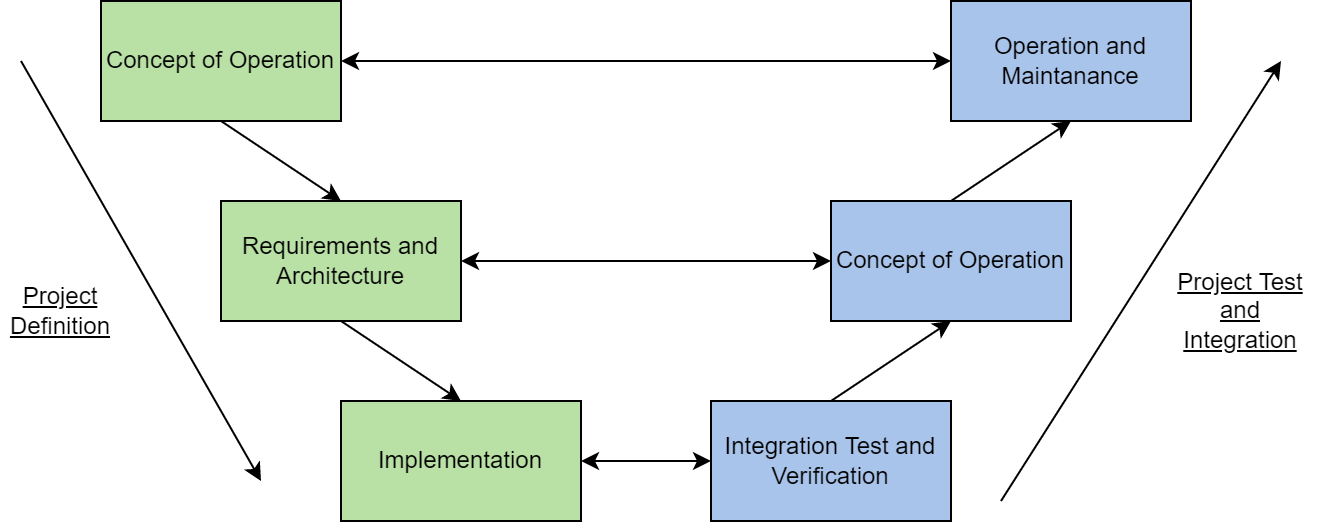
\includegraphics[width=\columnwidth]{V-Model.png}
    \caption{The V-Model helps in an IT-Project to have a focus on planning and implementation while reflecting and testing the program.}
    \label{fig:V-Model}
\end{figure}

\subsection{Scrum} \label{sec:Planning Method: Scrum}

\section{Architecture Design} \label{sec:Architecture Design}
\begin{itemize}
    \item Beschreibt Architektur von ROS
    \item UML Klassendiagram
    \item Interfaces für Messages
    \item Kommunikationsdiagramm (zwischen Algorithmen)
\end{itemize}

\section{Exploration Algorithm} \label{sec:Exploration Algorithm}
To find the middle line an algorithm has to be used. The exploration algorithm finds the line on which the car should drive on the first round on the track. Exploration is possible with the help of the current position of the car and the cones which are recognized by the Lidar sensor and stereo camera while the car is moving along the track. The \acrshort{ros} Node ``/path\_planner'' subscribes on the ``cone'' and ``current\_position'' topic where it gets all the information needed to calculate the path. For the subscription of ``/current\_position'' a callback function named ``self.\_\_current\_position\_listener\_callback'' will save the position in a local variable. The ``cone'' subscription listens to new cones that will be published via the ``cone\_publisher'' Node.

\section{Optimization Algorithm} \label{sec:Optimization Algorithm}
After the explore algorithm analysed the middle line of the track the board computer switches to the optimization algorithm. For the base code of the algorithm we forked the code from \acrlong{tum} (\acrshort{tum}). \cite{tumftm_optimization_algoritm} 



\section{V-Model}
\lipsum[1]